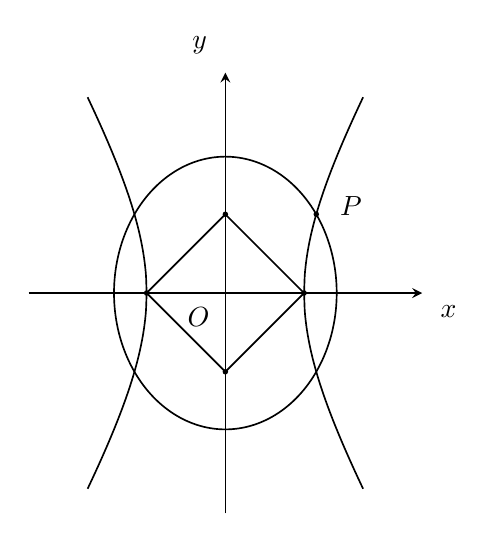
\begin{tikzpicture}[x=1cm,y=1cm,line width=0.6pt]
\coordinate (O) at (0,0);
\coordinate (Vright) at (1,0);
\coordinate (Vleft) at (-1,0);
\coordinate (Vtop) at (0,1);
\coordinate (Vbot) at (0,-1);
\coordinate (P) at (1.1547,1);
% axes
\draw[-stealth] (-2.5,0) -- (2.5,0);
\draw[-stealth] (0,-2.8) -- (0,2.8);
% ellipse C2: x^2/2 + y^2/3 = 1
\draw plot[domain=0:360,samples=200,smooth] ({1.41421356*cos(\x)},{1.73205081*sin(\x)});
% hyperbola C1: x^2 - y^2/3 = 1, right branch
\draw plot[domain=1:1.75,samples=100,smooth] ({\x},{1.73205081*sqrt(\x*\x-1)});
\draw plot[domain=1:1.75,samples=100,smooth] ({\x},{-1.73205081*sqrt(\x*\x-1)});
% left branch
\draw plot[domain=1:1.75,samples=100,smooth] ({-\x},{1.73205081*sqrt(\x*\x-1)});
\draw plot[domain=1:1.75,samples=100,smooth] ({-\x},{-1.73205081*sqrt(\x*\x-1)});
% central diamond (square) with vertices (pm1,0),(0,pm1)
\draw (Vright) -- (Vtop) -- (Vleft) -- (Vbot) -- cycle;
% dots at diamond vertices on axes
\fill (Vright) circle (0.035);
\fill (Vleft) circle (0.035);
\fill (Vtop) circle (0.035);
\fill (Vbot) circle (0.035);
\fill (P) circle (0.035);
% labels with clearance (O placed away from axes and diamond edges)
\node[below right,xshift=3pt,yshift=-1pt] at (2.5,0) {$x$};
\node[above left,xshift=-3pt,yshift=3pt] at (0,2.8) {$y$};
\node at (-0.34,-0.30) {$O$};
\node[right,xshift=5pt,yshift=3pt] at (P) {$P$};
\end{tikzpicture}
